\documentclass[french,12pt]{report}


\usepackage{hyperref}
\usepackage{graphicx}
\usepackage{currfile}
\usepackage{fancyhdr}
\usepackage[ddmmyyyy]{datetime}
\usepackage{geometry}
\geometry{hmargin=3.5cm,vmargin=3cm}
\usepackage{indentfirst}
\usepackage[utf8]{inputenc}
\usepackage{placeins}


\pagestyle{fancy}

\renewcommand{\headrulewidth}{1pt}
\fancyhead[C]{} 
\fancyhead[L]{\textit{Récupération, intégration et analyse de données géoréférencées}}
\fancyhead[R]{}

\renewcommand{\footrulewidth}{1pt}
\fancyfoot[C]{Cahier des charges} 
\fancyfoot[L]{\today\ }
\fancyfoot[R]{\thepage}

% Rename the auto titles
\renewcommand{\chaptername}{Chapitre}
\renewcommand{\contentsname}{Table des matières}

\renewcommand{\familydefault}{\sfdefault}

\begin{document}
\begin{normalsize}

	\thispagestyle{empty}
	

   \begin{figure}[!h]
	\centerline{
\includegraphics[width=7cm]{ifsttar.png}}	
   \end{figure}

    
    \begin{minipage}[c]{.46\linewidth}
     \begin{center}
             
\includegraphics[width=3cm]{iut_nantes.png}
         \end{center}
   \end{minipage} \hfill
   \begin{minipage}[c]{.46\linewidth}
    \begin{center}
            
\includegraphics[width=3cm]{iut_info_nantes.png}
        \end{center}
 \end{minipage}
 \vspace{2.5cm}
 	\begin{center}

 	
 	\begin{huge}
	Cahier des charges fonctionnel\\
	\end{huge}
	\vspace{0.75cm}
	\begin{large}
	\textit{Récupération, intégration et analyse de données géo-référencées} 
	\end{large}	
	\end{center}
 	\begin{center}
 	 \vspace{1cm}
Institut Universitaire de Technologie de Nantes\\
\vspace{0.5cm}

4 mai 2018\\
\vspace{3cm}
\begin{tabular}{ll}
\textbf{Stagiaire} & Florian DANIEL \\
\textbf{Tuteurs} & Pascal GASTINEAU\\
& Pierre HANKACH \\
\textbf{Suivi} & Solen Quiniou \\
\end{tabular}


\end{center}
 

\tableofcontents


   \chapter{Généralités}
   
   \section{Problématique}
Depuis quelques années, le numérique prend une place de plus en plus importante au sein de nos sociétés. Cet avènement soudain se caractérise particulièrement par la mise à disposition des données récoltées notamment par les autorités publiques : c’est l’Open Data. Ce type de données constitue un élément important dans ce projet, puisqu’il est à l’origine même de son existence. 


\noindent \\De nombreuses disparités existent entre ces données, cependant elles ont toutes un point commun : elles sont disponibles sur Internet.


   \section{Finalités}


L’objectif du projet est de créer un ensemble d’outils nécessaires à l’exploitation de données géo-référencées, sous forme de librairies. Le résultat du travail est à destination d’un institut public de recherche, l’IFSTTAR. 
Les informations, provenant de plusieurs sources (\textit{INSEE}\footnote{Institut National de la Statistique et des Études Économiques}, \textit{data.gouv}), il est essentiel de récupérer les données sur Internet, de les nettoyer afin d’obtenir des informations manipulables par programmation. Enfin, il s’agit de les intégrer dans une structure organisée : une \textbf{base de données}.  Ensuite, l’utilisateur aura la possibilité d’effectuer des requêtes, des modifications de données en grand volume comme une reprojection spatiale\footnote{Ré-exprimer des coordonnées géographiques dans un autre référentiel cartographique} .
\\

Ce processus est obligatoire pour toute information transitant par le programme. Il garantira l’\textbf{intégrité} et la \textbf{cohérence} des données en bases afin de les rendre le plus facilement exploitables par les utilisateurs.
\\

Le projet sera destiné à un ensemble d’utilisateurs, ne disposant pas nécessairement d'une connaissance approfondie du logiciel. La solution s’appuiera donc sur une \textbf{documentation claire} et \textbf{concise}, qui participera grandement à la compréhension. Le produit devra également répondre à certaines exigences du client quant à sa modularité, sa maintenabilité et sa facilité d’utilisation.\\

Les outils mis à disposition, à la fin du projet, devront permettre à l’utilisateur de garder une certaine indépendance afin qu’il puisse les utiliser selon son gré, tout en gardant une légère automatisation, dans le but de lui faire gagner du temps. la librairie constituera donc une assistance à la récupération et à l’analyse de données.  
\begin{figure}[h]
	\centerline{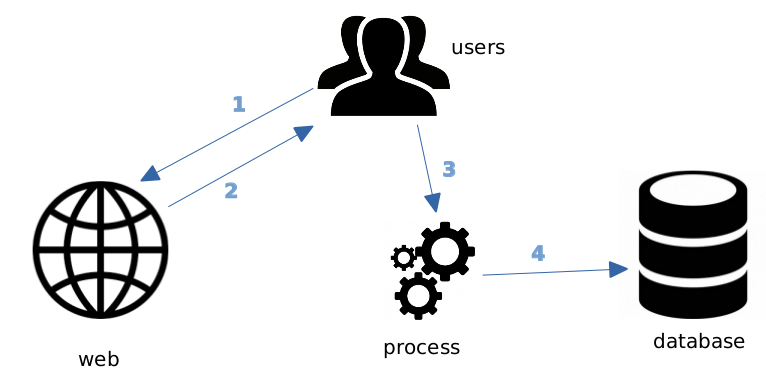
\includegraphics[width=10cm]{diagram.png}}
	\caption{Schéma de fonctionnement}
 \end{figure}

\begin{scriptsize}
\noindent (1) Requête d'un fichier via URL\\
(2) Récupération d'un fichier via HTTP\\
(3) Préparation et transformation des données\\
(4) Intégration des informations en base de données
\end{scriptsize}

   \section{Parties concernées par le projet}
   L’institut "client" relaie et stocke de nombreuses informations géographiques de différents formats (.shape, .dbf, .shx …), représentant un volume de données très conséquent, afin de les rendre graphiquement interprétable.
\\

Monsieur Gastineau et Monsieur Hankach, les tuteurs du stage, ont énoncé leur besoin. Le projet concerne actuellement le département "Aménagement, mobilités et environnement" (AME), et plus particulièrement le laboratoire "Environnement-Aménagement, Sécurité et Eco-conception" (EASE).
\\ 

Madame Quiniou est la professeure référente de l’IUT de Nantes pour ce stage. Elle veillera à la compatibilité entre les objectifs pédagogiques de l’enseignement et la problématique technique.

\noindent \\Les parties participeront à l’évaluation finale de la solution, ponctué par une soutenance orale du stagiaire, fin juin.

   \section{Étude déjà menée}
   
\sloppy Un étudiant en DUT Informatique (IUT de Nantes), Rémi TAUNAY, avait déjà réalisé, l’année dernière, un projet portant sur une solution d’automatisation répondant à la problématique de récupération, d'intégration et d'analyse de données 
géo-référencées\footnote{Rémi TAUNAY, 2017, Cahier des charges, \textit{Développement d'un outil de création de bases de données géo-référencées}}.
\\

Son travail est de bonne qualité mais instable du fait de l’\textbf{incompatibilité des versions actuelles} des logiciels.
Nous nous contenterons seulement de reprendre son travail d’installation des logiciels, ainsi que certaines fonctionnalités que le stagiaire avait implémenté. Nous respecterons donc ses choix logiciels et techniques afin de s’assurer d’être dans la continuité de son travail. 

\noindent \\Les études antérieures ont eu une incidence sur le besoin actuel, énoncé par le client. 

   
   
   \chapter{Des besoins, une solution}
   
   \section{Besoin exprimé}
   Les études menées précédemment, ont eu un large impact sur la forme que doit prendre la solution finale. Cette année, il s’agit de créer un ensemble de méthodes et d’outils, plus précisément une librairie, ayant pour but de réaliser les missions suivantes: 
   \begin{itemize}
\item un \textbf{pré-traitement}, consistant au téléchargement sur le réseau Internet, l’extraction d’archives, et l’organisation des fichiers dans l’arborescence.
\item une \textbf{prévisualisation des données} présentées dans le fichiers bruts.
\item un \textbf{traitement} regroupant le nettoyage des données ainsi que les opérations de configuration et de requêtes sur la base de données.
\end{itemize}
   
   \noindent \\La finalité requiert également plusieurs qualités, chères à l’utilisateur :
      \begin{itemize}
\item \textbf{fiable} : service n’échouant jamais à sa mission principale.
\item \textbf{intuitif} : choix de noms des méthodes adaptés, ...
\item \textbf{personnalisable} : malléable à toute structure/architecture informatique. Choix du dossier de destination, ...
\item \textbf{maintenable} : guide d’installation, prise en charge des exceptions, document de maintenance en cas de problème sévère, ...
\end{itemize}
   \section{Solution proposée}
   La solution prendra donc la forme d’une librairie en langage de programmation Python, car celui-ci confère de nombreux avantages quant à sa rapidité d'exécution et de traitement de données. Cet ensemble sera accompagné d’une documentation claire et lisible, afin de faciliter le processus de compréhension pour l’utilisateur.
\\
\noindent Les packages seront détaillés dans le chapitre suivant \hyperref[cadre-technique]{“Cadre technique”}.

   \section{Complexité}
   
\noindent La complexité du projet étudié est due à de nombreux paramètres :
   \begin{itemize}
\item la \textbf{diversité des sources d’informations}. En effet, les utilisateurs procéderont à la récupération de données issues de l’\textit{INSEE}, \textit{data.gouv}, sources étrangères. Ces organismes ont tendance à ajouter des éléments (image, source,tableaux à formes originales, …), que l’on peut considérer comme “parasites”. Ceux-ci peuvent entraîner une mauvaise réaction d’un programme et ainsi complexifier le travail des utilisateurs.

\item  les \textbf{utilisations du programmes très variées}, qui nécessite la prise en compte de nombreux facteurs
\item la \textbf{gestion des erreurs}. Elle faisait défaut dans les projets précédents, elle doit être un élément central de la solution.
\end{itemize}
   \chapter{Cadre technique}\label{cadre-technique}
   \noindent \textit{Les fonctions suivantes seront intégralement réalisées en Python}.
   \section{Pré-traitement}
\noindent \textit{Ce module comportera tous les outils ayant un lien avec la récupération des données ou le processus de pré-transformation.}\\


\texttt{download} : télécharger un fichier via HTTP grâce à son URL.\\

\texttt{extract} : vérifier si un fichier est une archive.\\

\texttt{isCompressed} : extraire une archive.\\

\texttt{fileInfo} : récapituler les informations d’un fichier (nom, extension, taille, nombre de feuilles Excel, …).\\

 


   \section{Traitement}
   
\noindent \textit{Ce module comportera toutes les méthodes ayant un lien avec la transformation ou la prévisualisation des données}\\

   Dans les fonctions suivantes, pour chaque méthode, il y a trois comportements différents : les fichiers Excel (tableurs), les données brutes (csv) et les données géographiques (.shape, .dbf). Nous nous appuierons sur différents librairies telles que \texttt{pandas} pour l’affichage ou \texttt{xlrd} pour la lecture de fichiers Excel.\\
   
   \texttt{dataView} : visionner une partie d’un jeu de données, sous forme de tableau. Plusieurs paramètres sont disponibles comme la plage de lignes, de colonnes, une feuille précise.\\
   
   \texttt{dataInfo} : récolter des informations sur un jeu de données comme le nombre de lignes et de colonnes, la projection s’il s’agit d’un fichier géographique. Sélectionner un sous-ensemble de données dans un tableau.
   
   \section{Intégration en base de données}
\noindent \textit{Ce module comportera tous les outils nécessaires à la manipulation des informations pour les bases de données}\\   
   
  Dans ce module, on utilisera une base de données \texttt{PostgresSQL}, avec l’extension géographique \texttt{PostGIS}. Afin de manipuler, les données, nos utiliserons surtout la librairie \texttt{sqlalchemy}.\\
  
     \texttt{inMemory} :représenter un ensemble de données brutes, provenant d’un tableur, sous forme de structure de données (\textit{dataframe}).\\
     
     \texttt{toDatabase} : importer/insérer des informations et des données en base de données.\\
     
     \texttt{fromDatabase} : exporter des informations d’une bases de données, quelque soit leurs sources.\\

     \texttt{reprojection} : effectuer une reprojection spatiale sur les données géographiques dans une table.\\
   \section{Tests unitaires}
   Nous effectuerons également des tests unitaires et paramétriques, en utilisant le module de test OpenSource de \href{https://github.com/wolever/parameterized}{\textit{wolever}} : \texttt{parameterized}, basé sur \texttt{nosetests}.\\
   
   \noindent Ce processus a pour but de garantir l'intégrité et la fiabilité des résultats obtenus.
   \chapter{Organisation}
   \section{Planification}
   Vous trouverez ci-dessous, un aperçu du diagramme de Gantt servant de référence pour l'organisation.

   
   \begin{figure}[!h]
	\centerline{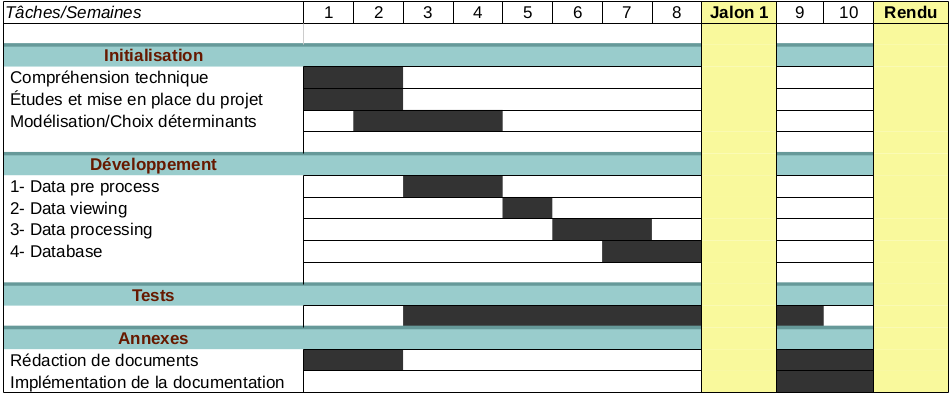
\includegraphics[width=15cm]{gantt_def.png}}
	\caption{Diagramme de Gantt}
   \end{figure}
      

  \section{Structure du projet}
\begin{figure}[h]
	\centerline{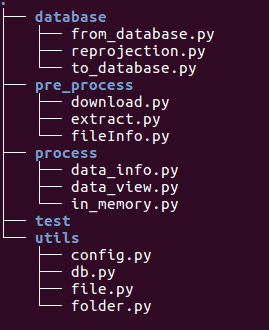
\includegraphics[width=5cm]{tree.png}}
	\caption{Structure globale des fichiers}
 \end{figure}     
\FloatBarrier


 \section{Évaluation du produit}
 Afin de garantir, la satisfaction cliente, il est nécessaire d’imposer des critères d’évaluations, afin de définir les fonctionnalités à retravailler, et celles qui correspondent au besoin exprimé. Les critères suivants seront évalués dans une durée comprise entre 20 min et 1 heure, dans un soucis de temps :
 
       \begin{itemize}
\item \textbf{fiabilité} : on reportera le nombre de fois où le programme n’a pas exécuté la demande de   l’utilisateur. S’il s’agit d’une erreur de manipulation de l’utilisateur, celle-ci est aussi pris en compte (la cause étant alors la mauvaise documentation)
\item \textbf{maintenabilité} : si la solution rencontre un problème, l’utilisateur doit être capable de le résoudre. On comptera le nombre de tentatives.
\item \textbf{personnalisation} : l’utilisateur tentera d’utiliser le produit dans plusieurs contextes différents. La solution aura obligation d’être compatible.
\item \textbf{automatisation} : l’utilisateur ne doit pas trouver l’utilisation des méthodes fastidieuses. Si cela est le cas, l’automatisation n’a pas été assez approfondie.
\end{itemize}

\end{normalsize}
\end{document}
